\documentclass{ximera}
%\usepackage{todonotes}

\newcommand{\todo}{}

\usepackage{tkz-euclide}
\tikzset{>=stealth} %% cool arrow head
\tikzset{shorten <>/.style={ shorten >=#1, shorten <=#1 } } %% allows shorter vectors

\usepackage{tkz-tab}  %% sign charts
\usetikzlibrary{decorations.pathreplacing} 

\usetikzlibrary{backgrounds} %% for boxes around graphs
\usetikzlibrary{shapes,positioning}  %% Clouds and stars
\usetikzlibrary{matrix} %% for matrix
\usepgfplotslibrary{polar} %% for polar plots
\usetkzobj{all}
\usepackage[makeroom]{cancel} %% for strike outs
%\usepackage{mathtools} %% for pretty underbrace % Breaks Ximera
\usepackage{multicol}

\usepackage{polynom}



\usepackage[many]{tcolorbox}  %% for titled boxes
\newtcolorbox{xbox}[1]{%
    tikznode boxed title,
    enhanced,
    arc=0mm,
    interior style={white},
    attach boxed title to top center= {yshift=-\tcboxedtitleheight/2},
    fonttitle=\bfseries,
    colbacktitle=white,coltitle=black,
    boxed title style={size=normal,colframe=white,boxrule=0pt},
    title={#1}}


\usepackage{array}
\setlength{\extrarowheight}{+.1cm}   
\newdimen\digitwidth
\settowidth\digitwidth{9}
\def\divrule#1#2{
\noalign{\moveright#1\digitwidth
\vbox{\hrule width#2\digitwidth}}}





\newcommand{\RR}{\mathbb R}
\newcommand{\R}{\mathbb R}
\newcommand{\N}{\mathbb N}
\newcommand{\Z}{\mathbb Z}

%\renewcommand{\d}{\,d\!}
\renewcommand{\d}{\mathop{}\!d}
\newcommand{\dd}[2][]{\frac{\d #1}{\d #2}}
\newcommand{\pp}[2][]{\frac{\partial #1}{\partial #2}}
\renewcommand{\l}{\ell}
\newcommand{\ddx}{\frac{d}{\d x}}
\newcommand{\ddt}{\frac{d}{\d t}}

\newcommand{\zeroOverZero}{\ensuremath{\boldsymbol{\tfrac{0}{0}}}}
\newcommand{\inftyOverInfty}{\ensuremath{\boldsymbol{\tfrac{\infty}{\infty}}}}
\newcommand{\zeroOverInfty}{\ensuremath{\boldsymbol{\tfrac{0}{\infty}}}}
\newcommand{\zeroTimesInfty}{\ensuremath{\small\boldsymbol{0\cdot \infty}}}
\newcommand{\inftyMinusInfty}{\ensuremath{\small\boldsymbol{\infty - \infty}}}
\newcommand{\oneToInfty}{\ensuremath{\boldsymbol{1^\infty}}}
\newcommand{\zeroToZero}{\ensuremath{\boldsymbol{0^0}}}
\newcommand{\inftyToZero}{\ensuremath{\boldsymbol{\infty^0}}}



\newcommand{\numOverZero}{\ensuremath{\boldsymbol{\tfrac{\#}{0}}}}
\newcommand{\dfn}{\textbf}
%\newcommand{\unit}{\,\mathrm}
\newcommand{\unit}{\mathop{}\!\mathrm}
\newcommand{\eval}[1]{\bigg[ #1 \bigg]}
\newcommand{\seq}[1]{\left( #1 \right)}
\renewcommand{\epsilon}{\varepsilon}
\renewcommand{\iff}{\Leftrightarrow}

\DeclareMathOperator{\arccot}{arccot}
\DeclareMathOperator{\arcsec}{arcsec}
\DeclareMathOperator{\arccsc}{arccsc}
\DeclareMathOperator{\si}{Si}
\DeclareMathOperator{\proj}{proj}
\DeclareMathOperator{\scal}{scal}


\newcommand{\tightoverset}[2]{% for arrow vec
  \mathop{#2}\limits^{\vbox to -.5ex{\kern-0.75ex\hbox{$#1$}\vss}}}
\newcommand{\arrowvec}[1]{\tightoverset{\scriptstyle\rightharpoonup}{#1}}
\renewcommand{\vec}{\mathbf}
\newcommand{\veci}{\vec{i}}
\newcommand{\vecj}{\vec{j}}
\newcommand{\veck}{\vec{k}}
\newcommand{\vecl}{\boldsymbol{\l}}

\newcommand{\dotp}{\bullet}
\newcommand{\cross}{\boldsymbol\times}
\newcommand{\grad}{\boldsymbol\nabla}
\newcommand{\divergence}{\grad\dotp}
\newcommand{\curl}{\grad\cross}
%\DeclareMathOperator{\divergence}{divergence}
%\DeclareMathOperator{\curl}[1]{\grad\cross #1}


\colorlet{textColor}{black} 
\colorlet{background}{white}
\colorlet{penColor}{blue!50!black} % Color of a curve in a plot
\colorlet{penColor2}{red!50!black}% Color of a curve in a plot
\colorlet{penColor3}{red!50!blue} % Color of a curve in a plot
\colorlet{penColor4}{green!50!black} % Color of a curve in a plot
\colorlet{penColor5}{orange!80!black} % Color of a curve in a plot
\colorlet{fill1}{penColor!20} % Color of fill in a plot
\colorlet{fill2}{penColor2!20} % Color of fill in a plot
\colorlet{fillp}{fill1} % Color of positive area
\colorlet{filln}{penColor2!20} % Color of negative area
\colorlet{fill3}{penColor3!20} % Fill
\colorlet{fill4}{penColor4!20} % Fill
\colorlet{fill5}{penColor5!20} % Fill
\colorlet{gridColor}{gray!50} % Color of grid in a plot

\newcommand{\surfaceColor}{violet}
\newcommand{\surfaceColorTwo}{redyellow}
\newcommand{\sliceColor}{greenyellow}




\pgfmathdeclarefunction{gauss}{2}{% gives gaussian
  \pgfmathparse{1/(#2*sqrt(2*pi))*exp(-((x-#1)^2)/(2*#2^2))}%
}


%%%%%%%%%%%%%
%% Vectors
%%%%%%%%%%%%%

%% Simple horiz vectors
\renewcommand{\vector}[1]{\left\langle #1\right\rangle}


%% %% Complex Horiz Vectors with angle brackets
%% \makeatletter
%% \renewcommand{\vector}[2][ , ]{\left\langle%
%%   \def\nextitem{\def\nextitem{#1}}%
%%   \@for \el:=#2\do{\nextitem\el}\right\rangle%
%% }
%% \makeatother

%% %% Vertical Vectors
%% \def\vector#1{\begin{bmatrix}\vecListA#1,,\end{bmatrix}}
%% \def\vecListA#1,{\if,#1,\else #1\cr \expandafter \vecListA \fi}

%%%%%%%%%%%%%
%% End of vectors
%%%%%%%%%%%%%

%\newcommand{\fullwidth}{}
%\newcommand{\normalwidth}{}



%% makes a snazzy t-chart for evaluating functions
%\newenvironment{tchart}{\rowcolors{2}{}{background!90!textColor}\array}{\endarray}

%%This is to help with formatting on future title pages.
\newenvironment{sectionOutcomes}{}{} 



%% Flowchart stuff
%\tikzstyle{startstop} = [rectangle, rounded corners, minimum width=3cm, minimum height=1cm,text centered, draw=black]
%\tikzstyle{question} = [rectangle, minimum width=3cm, minimum height=1cm, text centered, draw=black]
%\tikzstyle{decision} = [trapezium, trapezium left angle=70, trapezium right angle=110, minimum width=3cm, minimum height=1cm, text centered, draw=black]
%\tikzstyle{question} = [rectangle, rounded corners, minimum width=3cm, minimum height=1cm,text centered, draw=black]
%\tikzstyle{process} = [rectangle, minimum width=3cm, minimum height=1cm, text centered, draw=black]
%\tikzstyle{decision} = [trapezium, trapezium left angle=70, trapezium right angle=110, minimum width=3cm, minimum height=1cm, text centered, draw=black]

\author{Bart Snapp\and Nela Lakos}
\license{Creative Commons 3.0 By-NC}
\acknowledgement{https://www.whitman.edu/mathematics/calculus/}
  \outcome{Interpret an optimization problem as the procedure used to make a system or design as effective or functional as possible.}
  \outcome{Set up an optimization problem by identifying the objective function and appropriate constraints.}
  \outcome{Solve optimization problems by finding the appropriate absolute extremum.}
  \outcome{Solve basic word problems involving maxima or minima.}
\begin{document}
\begin{exercise}

  You want to make cylindrical containers to hold 1 liter (1000$\text{cm}^3$) using the
  least amount of construction material.  The side is made from a
  rectangular piece of material, and this can be done with no material
  wasted.  However, the top and bottom are cut from squares of side
  $2r$, so that $2(2r)^2=8r^2$ of material is needed (rather than
  $2\pi r^2$, which is the total area of the top and bottom).  Find
  the dimensions of the container using the least amount of material.
  \begin{hint}
  The total  area of the material spent consists of the area of the lateral side of the cylinder plus the area of two squares of side $2r$.
  
  
  $S= 2\pi r h +8 r^2$

\begin{image}
    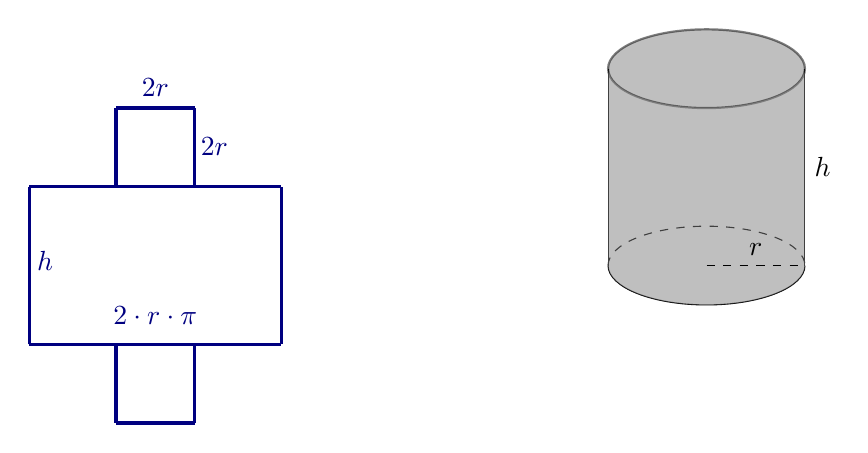
\begin{tikzpicture}
      \draw[very thick,penColor] (-1.6,0)  (0,2);% top half of ellipse
      \draw[penColor, very thick] (-1.6,-2) -- (1.6,-2);
      \draw[penColor, very thick] (1.6,-2) -- (1.6,0);
      \draw[penColor,very thick] (-1.6,-2) -- (-1.6,0);
      \draw[penColor,very thick] (-1.6,0) -- (1.6,0);
       \draw[penColor, very thick] (-0.5,-2) -- (-0.5,-3);
      \draw[penColor, very thick] (-0.5,-3) -- (0.5,-3);
      \draw[penColor,very thick] (0.5,-2) -- (0.5,-3);
      \draw[penColor,very thick] (-0.5,1) -- (0.5,1);
       \draw[penColor, very thick] (0.5,0) -- (0.5,1);
      \draw[penColor, very thick] (-0.5,0) -- (-0.5,1);
     \node [below,penColor] at (0.75,0.75) {$2r$};
       \node [below,penColor] at (0,1.5) {$2r$};
      \node [below,penColor] at (-1.4,-0.7) {$h$};
       \node [below,penColor] at (0,-1.4) {$2\cdot r\cdot \pi$};
       
        \draw [fill=gray,opacity=.5,thick](7,1.5) ellipse (1.25 and 0.5);
\draw (5.75,1.5) -- (5.75,-1);
\draw (5.75,-1) arc (180:360:1.25 and 0.5);
\draw [dashed] (5.75,-1) arc (180:360:1.25 and -0.5);
\draw (8.25,1.5) -- (8.25,-1) node[right,pos=.5]{$h$};  
\fill [gray,opacity=0.5] (5.75,1.5) -- (5.75,-1) arc (180:360:1.25 and 0.5) -- (8.25,1.5) arc (0:180:1.25 and -0.5);
\draw[dashed](5.75+1.25,-1) -- (8.25,-1) node[above,pos=.5] {$r$};
    \end{tikzpicture}
  \end{image}
  \end{hint}
  \begin{hint}
  Use the fact that the volume of the cylinder, $V=r^2\cdot\pi\cdot h$ and that $V=1000$.
  Express $h$ in terms of $r$.
  Now you can express $S$ as a function of $r$.
    \end{hint}
   Our objective function $S$ is given by the expression
   
   
    $S(r)=\frac{\answer{2000}}{r}+8r^{\answer{2}}$.
    \begin{hint}
    
    \end{hint}
  \begin{prompt}
  \[
  \text{radius}=\answer{5}\text{cm}\qquad\text{height}=\answer{40/\pi}\text{cm}
  \]
  \end{prompt}
\end{exercise}
\end{document}
